%\documentclass[%
	%draft
%	]{ijsra}
\def\IJSRAidentifier{\currfilebase} %<---- don’t change this!
%-------Title | Email | Keywords | Abstract-------------
\def\shorttitle{Meeting of the Society for Medieval Archaeology Student Colloquium}
\def\maintitle{\shorttitle}
\def\cmail{sarah.kerr@kuleuven.be}
%\def\keywords{}
%\def\keywordname{}%<--- redefine the name “Keywords“ in needed language
\def\abstract{}
%--------Author’s names------------
\def\authorone{Dr Sarah Kerr}
%-------Biographical information-------------
\def\bioone{Dr Sarah Kerr is a Research Fellow at Katholieke Universiteit Leuven, Belgium. She gained her PhD from Queen’s University Belfast, in archaeology. Her project explored lodging ranges in late medieval England. Her current interests are communal living in medieval Europe and making research accessible to the wider public. She is a Council Member and Membership Secretary for the Society for Medieval Archaeology, having previously acted as the Student Representative in 2014, which involved hosting the Student Colloquium at Queen’s University Belfast. }
%------University/Institution--------------
\def\affilone{Katholieke Universiteit Leuven, Belgium}
%\begin{document}
\IJSRAopening%<---- don’t change this!
%-------
\lettrine{T}{he} 2016 instalment of the Society for Medieval Archaeology student colloquium was organised by Marit Van Cant, PhD-fellow for the Research Foundation Flanders (FWO), and studying for her doctorate with Vrije Universiteit Brussel (supervisor Prof. Dr. Dries Tys) and the University of Sheffield (co-supervisor Prof. Dawn Hadley). 
The colloquium took place on \nth{3}–\nth{5} November, in Brussels (\cref{fig:Kerr_fig01}), including a fieldtrip to Walraversijde and Bruges. This is the seventh annual Society for Medieval Archaeology (SMA) student colloquium, following from the first at the University of Birmingham in 2010, then sequentially University of Cambridge, Cardiff University, University of Aberdeen, Queen’s University Belfast and University of Sheffield. The SMA established the student colloquium to create a platform for postgraduate students and early career archaeologists to present their research in a friendly environment, create networks with their peers across Europe, and learn about the wealth of research taking place in medieval archaeology. The overarching goal of the SMA is to further the study of the medieval period, and by establishing the colloquium, it fosters links and creates a healthy network of students who will in turn advance the discipline.

The conference began with a tour of the city of Brussels, accompanied by description from local host Prof. Dr. Dries Tys, from Vrije Universiteit Brussel. At first the medieval archaeology may not be apparent to a visitor of Brussels, however closer inspection revealed a rich palimpsest, from the thick \nth{14} century city walls, to the French Gothic Cathedral of St. Michael and St. Gudula, with Brabantine features. The tour culminated in the medieval Grand Place; the city square with highly-gilded buildings demonstrating multiple architectural styles, an embodiment of the diversity of Brussels and its visitors. The medieval square was rebuilt in the \nth{17} century, its connection to the past maintained through the retention of the plan: this introduced the delegates to this year’s conference theme of ‘connections’. 

\begin{figure}[!tb]
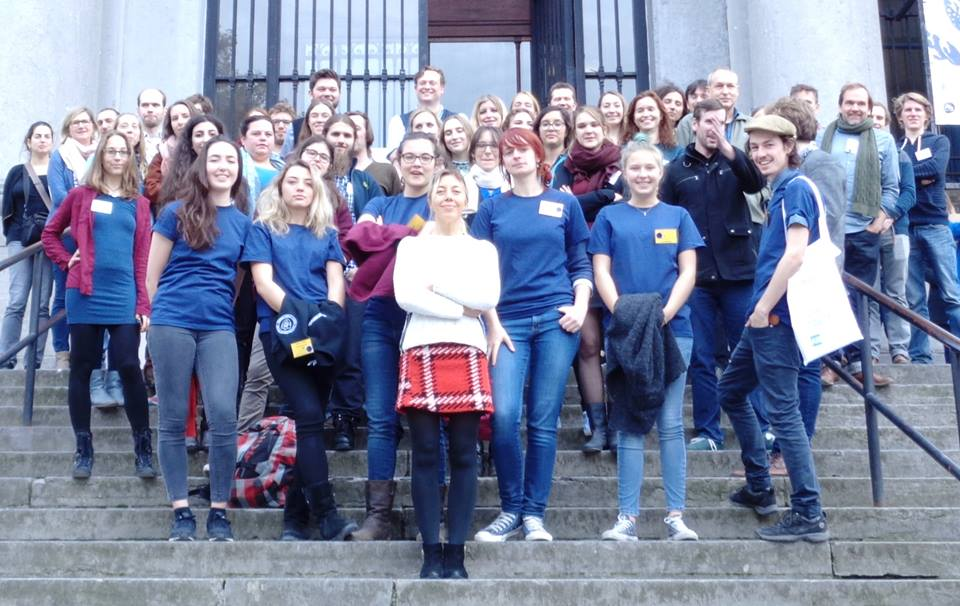
\includegraphics[width=\linewidth]{Kerr_fig01}
\caption{Participants of the colloquium, with organiser Marit Van Cant front and centre
        {\normalfont\scriptsize \\ \copyright\ by 
                 \shortauthor
                 % or NAME OF COPYRIGHT HOLDER
                  }}
\label{fig:Kerr_fig01}
\end{figure}
This comprehensive theme devised by Marit allowed postgraduate students and early career archaeologists to present on some element of their research; furthermore students from other disciplines but with a broader medieval significance could participate. Future themes are likely to retain a broad scope to allow as many contributions as the time allows, a range of paper topics, and an interdisciplinary aspect. 

The presentations took place in the Cinquantenaire Museum in the heart of Brussels; the delegates were well placed to explore further medieval archaeology in the museum’s collections during lunch breaks. Twenty-eight papers and posters were accepted which resulted in a wide range of topics pertaining to the theme of connections in the medieval period. This included the social connections visible in the archaeological record; such as the communication of ideas between Anglo-Saxon England and Alemannia, as discussed by Emma Bownlee (University of Cambridge). Temporal connections were considered by Indra Werthman (Durham University) who discussed the Roman objects and identity in Anglo-Saxon graves. Timothy Carlisle (University of Aberdeen) discussed the intangible connections to belief in his paper on house commemoration in Viking age Iceland. 

An important element of the conference is providing the opportunity for delegates to develop their presenting skills. Students get hands-on experience through practicing in front of their peers, and through watching an invited speaker of renowned importance, and this year’s keynote, Dr Anton Ervynck from Flanders Heritage Agency did not disappoint. His lively presentation, in the oldest bar in Brussels (\emph{A La Bécasse}), enlightened and entertained the delegates; with stories of excavating in the 1980s plus the trials and tribulations of research. Dr Ervynck is a biologist who started his scientific career by developing theoretical models for the feeding behaviour of oystercatchers. He shifted to palaeontology, producing a PhD at the University of Amsterdam about the distribution history of the black and brown rat. This brought him to the field of environmental archaeology where he is mainly studying Roman to postmedieval sites from Flanders. Field work abroad involved campaigns in Spain, Turkey, Egypt, Jordan and the Crimean Peninsula. Methodological work concentrated on the history of domestic pigs. A close collaboration with Wim Van Neer of the Royal Belgian Institute of Natural Sciences, resulted in a reconstruction of the development of marine fishery in the southern Low Countries. His paper titled ‘The Food that Mattered: A Reality Check on Changing Post-Roman Consumption Patterns’ discussed the southern low countries and how consumption patterns had changed over centuries. Our delegates learned that, a “reality check” is required at times during research as the results may be intriguing as well as surprising and confronting. 

Evening events are often planned for the colloquium, giving delegates the chance to network and discuss the day’s papers. Over the years students, delegates, and hosting academics alike have enjoyed Scottish cèilidh, Irish mead tasting, and conference dinners. This year, Marit organised a Belgian beer tasting evening following Dr Ervynck’s keynote, plus a conference dinner serving traditional Flemish dishes. As always, the social aspect was a highlight for the delegates as Marit received warm and grateful comments in the feedback.
The relaxed and friendly atmosphere of the colloquium is an asset as it allows presenters to develop their skills; however this year there was still an element of competition. Votes were cast for the best paper presentation and first place was awarded to Lance Pursey (University of Birmingham). The award was well deserved, as Lance brought the colloquium outside its European context with his paper discussing the Liao Empire of Northeast Asia. Second place was awarded to David Stone (University of Exeter) with his enthusiastic presentation on landscapes of defence in Anglo-Saxon England, and third prize went to Elisabeth Magin (University of Nottingham) for her paper with the intriguing title ‘“Gyda Tells You To Go Home”—Text Messaging and Archaeology'. 

The conference ended with what has become something of custom with the colloquium; a fieldtrip to local medieval sites. The delegates ventured to the coast of Belgium to Walraversijde, the reconstructed medieval village, which has been studied more thoroughly and more systematically than any other medieval fishing community in Europe, resulting in an reconstructed village and museum. The trip continued to Bruges, where Raakvlak, Intermunicipal Service for Archaeology, provided a modern tour of the famous city using tablets to include maps, documents, and pictures into the descriptive expedition. 
The student colloquium is a vital component of the SMA; its function is to provide a platform for students to share their research and, more importantly, create networks with peers across Europe and beyond. The network is the mainstay of the medieval archaeology community: through it future research is discussed, collaborative projects are planned and, of course, friendships are created. By joining the society and attending the colloquium (and other SMA events) the delegates maintain the medieval archaeology community while creating new connections across the continent and islands, regardless of boundaries and borders. This is one of the main achievements of the colloquium, as one delegate stated their favourite element was being part of a community of young medievalists in an international environment’. As the colloquium continues to grow and becomes a principal event in the academic calendar, the future of the discipline is outward looking and constructive.
Each year the Society for Medieval Archaeology invites a student member to take on the role of Student Representative. Organising the colloquium is the main task, plus attending the SMA council meetings and assisting with student membership. The call for a new student representative will be opened early in the year, watch the SMA website/ Facebook/ Twitter for the deadline. We encourage you to apply and hold the conference at your institution next year.

Thanks must go to Dr Anton Ervynck, assistants, sponsors, chairs, Vrije Universiteit Brussel, University of Sheffield, and most importantly to Marit for organising a fascinating and successful conference.


\IJSRAclosing%<---- don’t change this!
%%\end{document}